\documentclass[11pt,a4paper]{article}

\usepackage[dvips]{graphicx}
\input{/usr/local/lib/texmf/tex/dvips/psfig}
\input{/homes/arnaud/htdocs/latex2html/texinputs/html.sty}
\input{/homes/arnaud/htdocs/latex2html/texinputs/htmllist.sty}

% \htmlbase{http://denis.arnaud.free.fr/purdue/spa1}
\begin{latexonly}
  \renewcommand{\thefootnote}{\fnsymbol{footnote}}
  \renewcommand{\baselinestretch}{1.3}
\end{latexonly}

\newcommand{\con}{\rightarrow}
\newcommand{\cd}{\mbox{$\stackrel{d}{\rightarrow}$}}
\newcommand{\ep}{\varepsilon}
\newcommand{\hspaceo}{\mbox{\hspace{1cm}}}
\newcommand{\hspacet}{\mbox{\hspace{2cm}}}
\newcommand{\xh}{\hat{x}}
\newcommand{\xs}{x^{\star}}
\newcommand{\es}{e^{\star}}
\newcommand{\yh}{\hat{y}}
\newcommand{\xm}{x_m}
\newcommand{\xmh}{\hat{x}_m}
\newcommand{\ems}{e^{\star}_m}
\newcommand{\sjotm}{s_{j_1},s_{j_2},\cdots,s_{j_m}}
\newcommand{\sjom}{s_{j_1},\cdots,s_{j_m}}
\newcommand{\siot}{s_{i_1},s_{i_2}}
\newcommand{\A}{{\cal A}}
\newcommand{\X}{\{X_k\}}
\newcommand{\HX}{\hat{X}}
\newcommand{\tx}{\hat{x}}
\newcommand{\D}{{\cal D}}
\newcommand{\ie}{{\em i.e.}}
\newcommand{\eg}{{\em e.g.}}
\newcommand{\noi}{\noindent}
\newcommand{\parsec}{\par\noindent}
\newcommand{\med}{\medskip\parsec}
\newcommand{\gutter}{0.5in}
\newcommand{\basswidth}{3.413in}

\setlength{\textheight}{8.5in}
\setlength{\textwidth}{6.0in}

\begin{latexonly}
  \vsize=8.5in
  \voffset=-0.7in
  \hoffset=-0.4in
\end{latexonly}

\begin{document}

%\bodytext{BACKGROUND=../../background/grey.gif}
\bodytext{BODY BGCOLOR="#FFFFE8" LINK="#7B68EE" VLINK="#A9A9A9"}

\begin{center}
{\bf PATTERN MATCHING IMAGE COMPRESSION \\
WITH PREDICATION LOOP:\\
Preliminary Experimental Results}
\end{center}
\noi
\begin{tabular}{l@{\hspace{2in}}l}
Denis Arnaud&Wojciech Szpankowski\footnotemark\\
ENST& Department of Computer Science\\
46 Rue Barrault&Purdue University\\
75013 Paris&W. Lafayette, IN 47907\\
France&U.S.A.\\
{\tt darnaud@email.enst.fr}& {\tt spa@cs.purdue.edu}
\end{tabular}
\footnotetext{ This work was supported by NSF Grants NCR-9415491
and CCR-9201078.}

\vspace{2cm}

\centerline{\bf Abstract}

Recently, a novel image compression technique based on pattern matching was
proposed, namely {\it Pattern Matching Image Compression} (PMIC).
Basically, it is a lossy extension of the well known Lempel-Ziv scheme. It
was proved that such an extension leads to a suboptimal compression, and
that the compression ratio can as low as the so called R\'{e}nyi entropy.
Success of PMIC crucially depends on several enhancements such as searching
for reverse approximate matching, recognizing substrings in images that are
additively shifted versions of each other, introducing a variable and
adaptive maximum distortion level, and so forth. In this paper, we
introduce another enhancement, namely, predictive coding.  More precisely,
we implement {\it Differential Predictive Code Modulation} (DPCM) within
PMIC scheme. We report here some preliminary experimental results which
show that PMIC enhanced by DPCM can improve compression ratio for good
quality images as well as speed of compression for PMIC.
  
\begin{latexonly}
  \renewcommand{\thefootnote}{\arabic{footnote}}
  \setcounter{footnote}{0}
\end{latexonly}

\begin{htmlonly}
  \centerline{\htmladdnormallink{A Postscript version is also available
      here.}{http://denis.arnaud.free.fr/purdue/spa1.ps.gz}}
\end{htmlonly}

\newpage

\section{Introduction}

Since nowdays most media are represented in a digital form, it is natural
to apply a technique that was proved successful for inherently digital
media such as text, namely Lempel-Ziv type schemes (cf. \cite{zl1,zl2}).
In \cite{lus1,lus2} we propose to extend Lempel-Ziv approach to lossy
(approximate) compression. While it is know that the lossless Lempel-Ziv is
asymptotically optimal (i.e., its compression ratio is close to the
entropy), in \cite{lus2} \L uczak and Szpankowski (cf. also \cite{yk})
proved recently that a lossy extension of Lempel-Ziv scheme (of low
complexity) is suboptimal, that is, it attains the compression ratio equal
to the so called generalized R\'{e}nyi entropy (instead of the optimal
rate-distortion).\\

Using this theoretical underpinning, Atallah, genin and Szpankowski
\cite{ags} have recently implemented the above idea for image compression.
This novel scheme is called {\it Pattern Matching Image Compression}
(PMIC), and it is briefly review in the next section (see also \cite{cs}
for another implementation of a lossy Lempel-Ziv'78 scheme, however, there
is no theoretical justifications for the reported results).  In \cite{ags}
it was concluded that for images of good quality PMIC scheme is competitive
to JPEG and wavelet image compression.  Superiority of PMIC at
decompression (which does not require any computations since it basically
only reads data) may turn out to be a crucial advantage in practice where
asymmetric compression/decompression is a desirable feature (e.g., off-line
video).\\

The central theme of above approach is the notion of approximate
repetitiveness.  That is, if a portion of data almost-occurs five times,
perhaps in close proximity but not necessarily contiguously, then we need
only store the first such occurrence: The other four can be stored as
(direct or indirect) references to the first occurrence.  Somewhat
surprisingly, this theme of exploiting approximate repetitiveness is
uniformly useful to multimedia data, hence applies to text as well as to
image, video, and audio data.  However, the approximate repetitiveness can
be hidden in various forms for different types of media (so one must
consider different distortion measures).  This is in contrast with current
technology, where a different approach is used for each of these types of
data (e.g., text and images).  We plan to explore it in our future
research.\\

In \cite{ags} several {\it enhancements} were introduced to the basic idea
of PMIC that were instrumental for achieving good results. For example:
searching for reverse approximate matching, recognizing substrings in
images that are additively shifted versions of each other, introducing a
variable and adaptive maximum distortion level, and so forth.  These
enhancements are crucial to the overall quality of our scheme, and their
efficient implementation leads to algorithmic results of interest in their
own right. In this paper, we introduce one more enhancement, namely
prediction that -- as we shall see -- will lead to shorter compression time
and better compression ratio without significantly deterioration of image
quality. Actually, we propose a more ambitious plan, namely implementing
DPCM (\ie, Differential Predictive Code Modulation) within PMIC.\\

To see possible advantage of this new enhancement, we should observe that
differential image (composed of the difference between the original image
and its prediction) is much less correlated than the original one. Thus,
any compression algorithm should gain in performance when applied on the
differential image, instead of on the original one. However, for lossy
compression there is a need to perform a {\it prediction loop} as explained
in details in Section 3.  In DPCM, this prediction loop is performed on
each pixel, one by one. Thus, the implementation of a predictive feature
for such a scheme as PMIC needs a few adaptations, because PMIC treats
several pixels at a time, and does not work on a pixel-by-pixel basis.\\

The main idea to use a predictive loop in PMIC is that what is the basic
cell for DPCM, namely one pixel, becomes the longest prefix found in the
database for PMIC. As for DPCM, the differential image is quantized, thus
allowing a slight increase in the compression ratio. Besides, although a
differential image is significantly less correlated than the original
image, it is still slightly correlated. This is because the low-order,
linear predictor typically used here or in DPCM is suboptimal. But, while a
Huffman coding scheme would not take advantage of this remaining
correlation, since it encodes each differential value independently of its
neighboring values, the PMIC scheme does, because it is a context based
scheme. Thus, PMIC can achieve a bit rate potentially smaller than the
zeroth-oreder entropy of the differential image.  We report in this paper
our implementation and preliminary experimental results.

\section{Review of PMIC}

This section is based on Atallah {\it et al.} \cite{ags}.  The reader might
also want to consult \cite{lus1,lus2,sg,yk}.\\

The detection of the above-mentioned approximate repetitiveness is done by
approximate pattern matching, whence the name {\it Pattern Matching Image
  Compression} (PMIC).  The main idea behind it is a lossy extension of the
Lempel-Ziv data compression scheme in which one searches for the longest
prefix of an uncompressed file that {\it approximately} occurs in the
already processed file.  The distance measure subtending the notion of
approximate occurrence can be the {\it Hamming distance}, or of the {\it
  square error distortion}, or the {\em string edit} distance, or any of
the other distances considered in the distortion theory (cf.
\cite{berger}).\\

In short, let us consider a stationary and ergodic sequence
$\X_{k=1}^\infty$ taking values in a finite alphabet $\A$ (think of $\X$ as
an image scanned row by row). For image compression the alphabet $\A$ has
size $|\A|=256$.  We write $X_m^n$ to denote $X_mX_{m+1}\ldots X_n$, and
for simplicity $X^n = X_1 \ldots X_n$. The substring $X_1^n$ will be called
{\it database sequence} or {\it training sequence}.  We encode $X_1^n$ into
a compression code $C_n$, and the decoder produces an estimate $\HX_1^n$ of
$X_1^n$.  As a fidelity measure, we consider any distortion function
$d(\cdot, \cdot)$ that is subadditive, and that is a {\it single-letter
  fidelity} measures, that is, such that $ d(x^n,\tx^n)=\frac 1n
\sum_{i=1}^n d(x_i,\tx_i)$. Examples of fidelity measures satisfying the
above conditions are: {\it Hamming distance}, and the {\it square error
  distortion} where $d( x_i , \tx_i ) = (x_i -\tx_i)^2$.  As in \L uczak
and Szpankowski \cite{lus1,lus2} we define the depth $L_n$ as the length of
the longest prefix of $X_{n+1}^\infty$ (i.e., uncompressed image) that
approximately occurs in the database (i.e., already compressed image).
More precisely, for a given $0\leq D\leq 1$ we define: {\it Let $L_n$ be
  the length $k$ of the longest prefix of $X_{n+1}^\infty$ for which there
  exists $i$, $1\leq i\leq n-k+1$, such that
  $d(X_i^{i-1+k},X_{n+1}^{n+k})\leq D$} where $D$ is the maximum distortion
level.\\

A variable-length compression code can be designed based on $L_n$.  The
code is a pair ({\tt pointer to a position} $i$, {\tt length of} $L_n$), if
a sufficiently long $L_n$ is found. Otherwise we leave the next $L_n$
symbols uncompressed. We clearly need $\log n + \log L_n$ bits for the
above code.  The compression ratio $r$ can be approximated by

\begin{equation}
r={{\mathrm overhead~ information} \over {\mathrm
length ~of~repeated ~subword}}= {{\log n + \log L_n} \over L_n} ~,
\label{e2}
\end{equation}

and to estimate it one needs to find out probabilistic behavior of $L_n$.
In \cite{lus1,lus2} it is proved that $L_n \sim {1\over r_0(D)} \log n$
where $r_0(D)$ is the so called generalized R\'{e}nyi entropy (which could
be views as follows: the probability of a typical ball in $\A^n$ of radius
$D$ is approximately $2^{-n r_0(D)}$). From (\ref{e2}) we conclude that the
compression ratio $r$ is asymptotically equal to $r_0(D)$.\\

The above main idea is enhanced by several observations that constitute
PMIC scheme. They are:\\

{\bf Additive Shift}. It is reasonable to expect that in an image there are
several substrings, say $x^m$, $y^m$, that differ only by {\it almost}
constant pattern, that is, $y_i=x_i +c$ for $1\leq i \leq m$ where $c$ is
not necessary a constant, but whose variation is rather small.\\

In such a case we store the average difference $c$ as well as a
$(pointer,length)$ pair, which enables us to recover $y_i$ from $x_i$
(instead of storing $y_i$ explicitly).  In general, we determine the
additive shift $c$ by checking whether the following condition is fulfilled
or not

$$
{1\over m} \left(\sum_{i=1}^m (x_i-y_i)^2 -{1\over m} \left(\sum_{i=1}^m
(x_i-y_i)\right)^2 \right) \leq D'
$$

where $D'$ is a constant. If the above holds, we compute the shift $c$ as $
c={1\over m} \sum_{i=1}^m (x_i-y_i) $.  It can be easily verified that for
$x_i=y_i+c$, and $c$ a constant, the above procedure returns $c$. In
passing, we should observe that this enhancement improves even {\it
  lossless} ($D=0$) image compression based on the Lempel-Ziv scheme.\\

{\bf Reverse Prefix}. We check for similarities between a substring in the
uncompressed file and a {\it reversed} (i.e., read backward) substring in
the database.\\

{\bf Variable Maximum Distortion}.  It is well known that human vision can
easily distinguish an ``undesired'' pattern in a low frequency (constant)
background while the same pattern might be almost invisible to humans in
high frequency (quickly varying) background.\\

Therefore, we used a low value of maximum distortion, say $D_1$, for slowly
varying background, and a high value, say $D_2$, for quickly varying
background. We automatically recognize these two different situations by
using the derivative $\D_{ij}$ of the image that is defined as

$$
\D_{ij} ={(x_{i+1,j}-x_{ij})+(x_{i,j+1}-x_{ij}) \over 2}
$$

where $x_{ij}$ is the value of $(i,j)$ pixel.  In our implementation, we
used the lower value of $D$ whenever $\D_{ij}\leq 3$ and the higher value
of $D$ otherwise.\\

{\bf Max-Difference Constraint}.  Our code will also satisfy the additional
constraint that $| x_i - \tx_i | \leq DD$ where $DD$ is a suitably chosen
value. This additional constraint, which we call {\it max-difference}
constraint, ensures that visually noticeable ``spikes'' are not averaged
out of existence by the smoothing effect of the square error distortion
constraint.  We incorporate this max-difference constraint in the function
$d(\cdot , \cdot )$ by adopting the convention that $d( x_i , \tx_i ) = +
\infty$ if $| x_i - \tx_i | > DD$, otherwise $d( x_i , \tx_i )$ is the
standard distortion as defined above (i.e., Hamming or square of
difference).\\

{\bf Small Prefix}. It does not make too much sense to
store a $(pointer,position)$ when the longest prefix is small.
In this case, we store the original pixels of the image.\\

{\bf Run-Length Coding}. For those parts of the
picture that do not vary at all, or vary little,
we used run-length coding: if the next pixels vary little,
we store a pixel value and the number of repetitions.

\begin{latexonly}
  \begin{figure}
    \centerline{
      \psfig{file=lena_vR.ps,width=\basswidth}\hspace*{\gutter}
      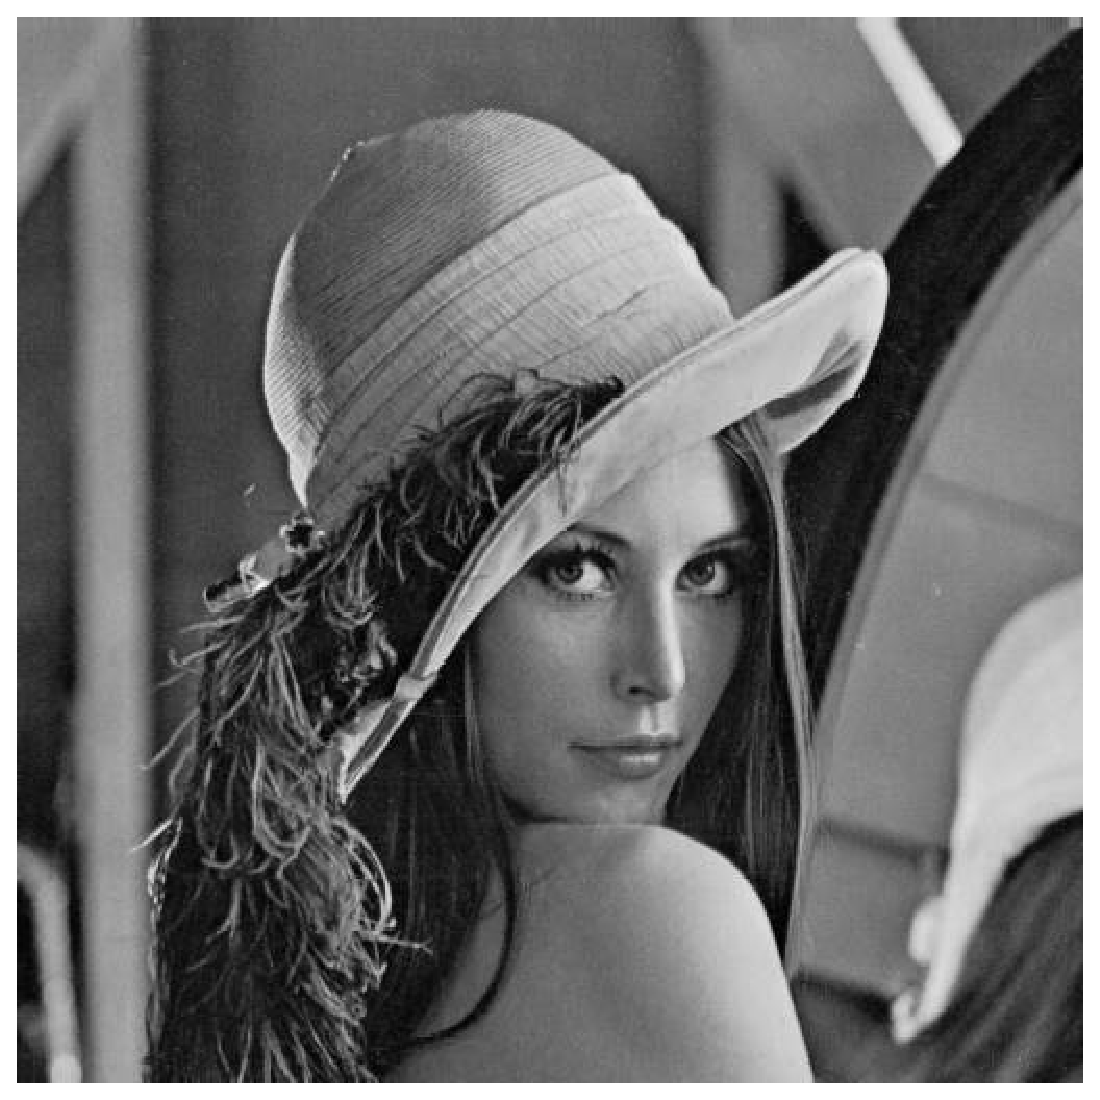
\psfig{file=lena_jpg.ps,width=\basswidth}}
    \centerline{\hbox to \basswidth{\hfill(a)\hfill}\hspace*{\gutter}
      \hbox to \basswidth{\hfill(b)\hfill}}
    
    \vspace{0.3in}

    \centerline{
      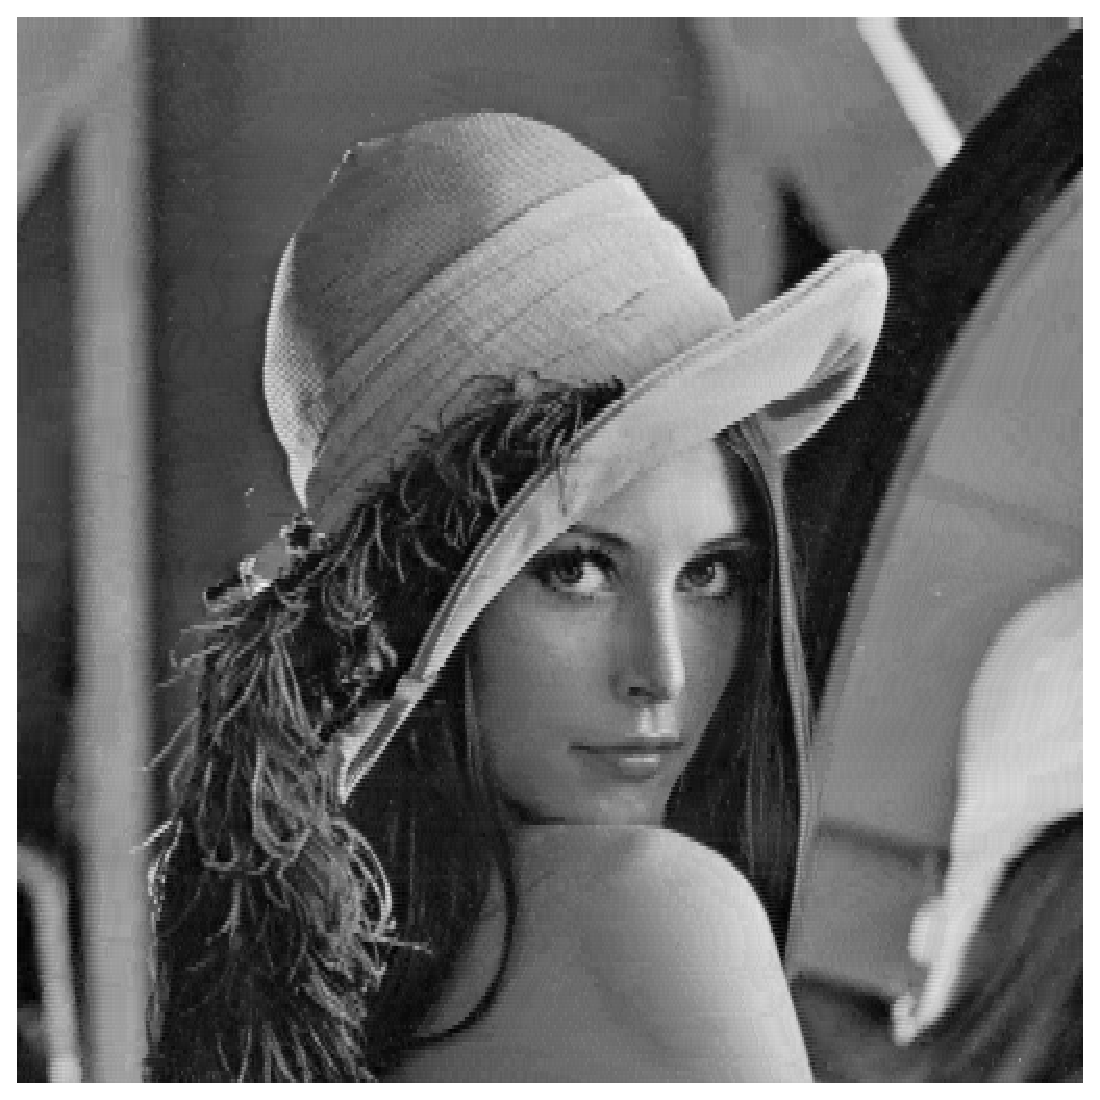
\psfig{file=lena_2b2.ps,width=\basswidth}\hspace*{\gutter}
      \psfig{file=lena_trans.ps,width=\basswidth}}
    \centerline{\hbox to \basswidth{\hfill(c)\hfill}\hspace*{\gutter}
      \hbox to \basswidth{\hfill(d)\hfill}}

    \caption[Different flavors of PMIC on the ``Lena'' image]{Comparisons
      of different flavors of PMIC on the ``Lena'' image:
      (a) Classical PMIC (compression ratio equal to 4.3);
      (b) JPEG (compression ratio equal to 7.9);
      (c) PMIC with simple predictive coding (compression ratio equal to
      7.9);
      (d) PMIC with column compression (compression equal to 5.3).}
\label{comp_lena_flavors}
\end{figure}
\end{latexonly}

\begin{htmlonly}
  \centerline{
    \psfig{file=lena_vR.ps,width=2in}
    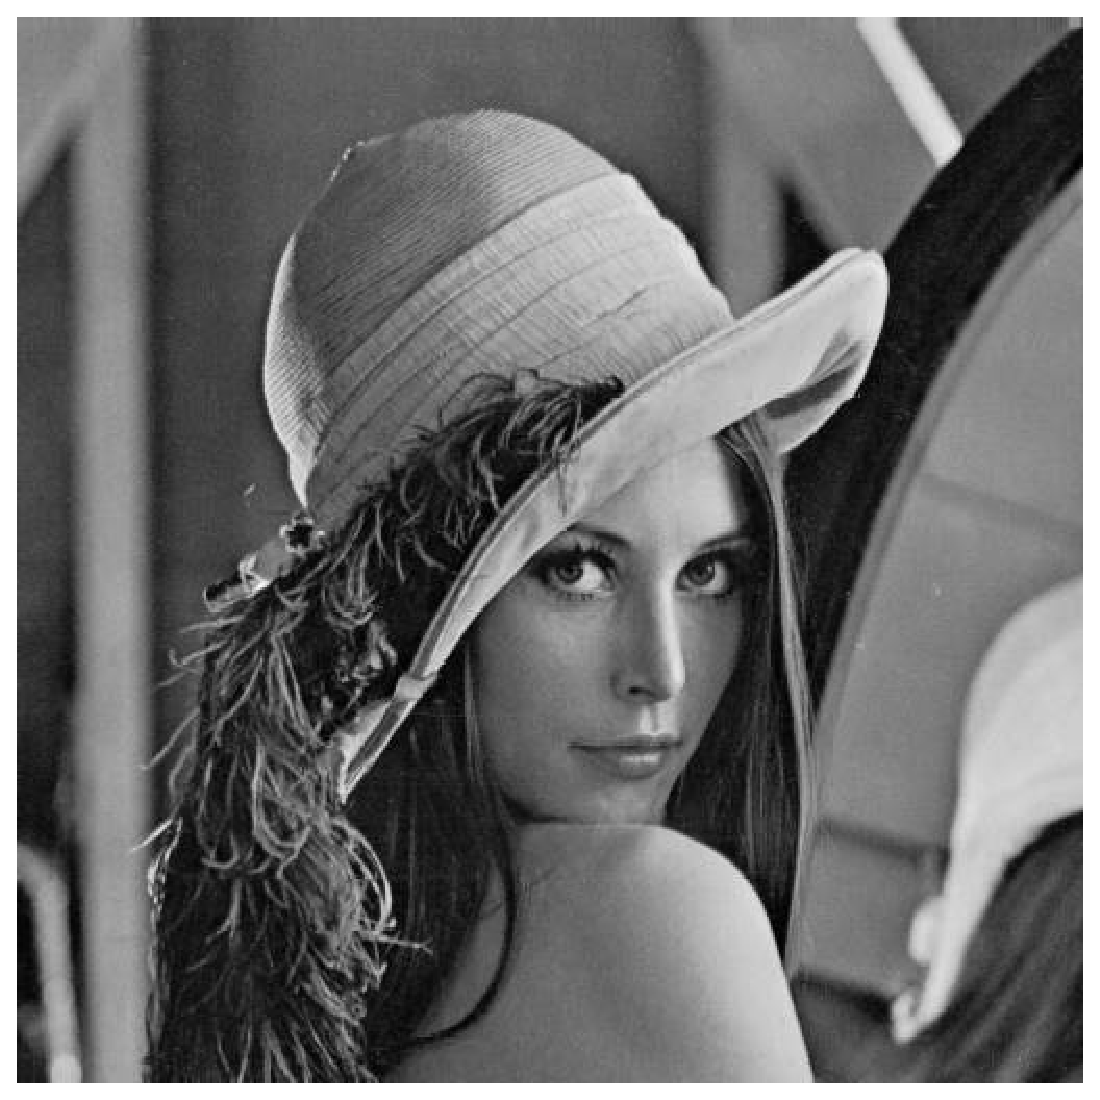
\psfig{file=lena_jpg.ps,width=2in}
    }
  \centerline{(a)\hspace{2cm}(b)}
  \centerline{
    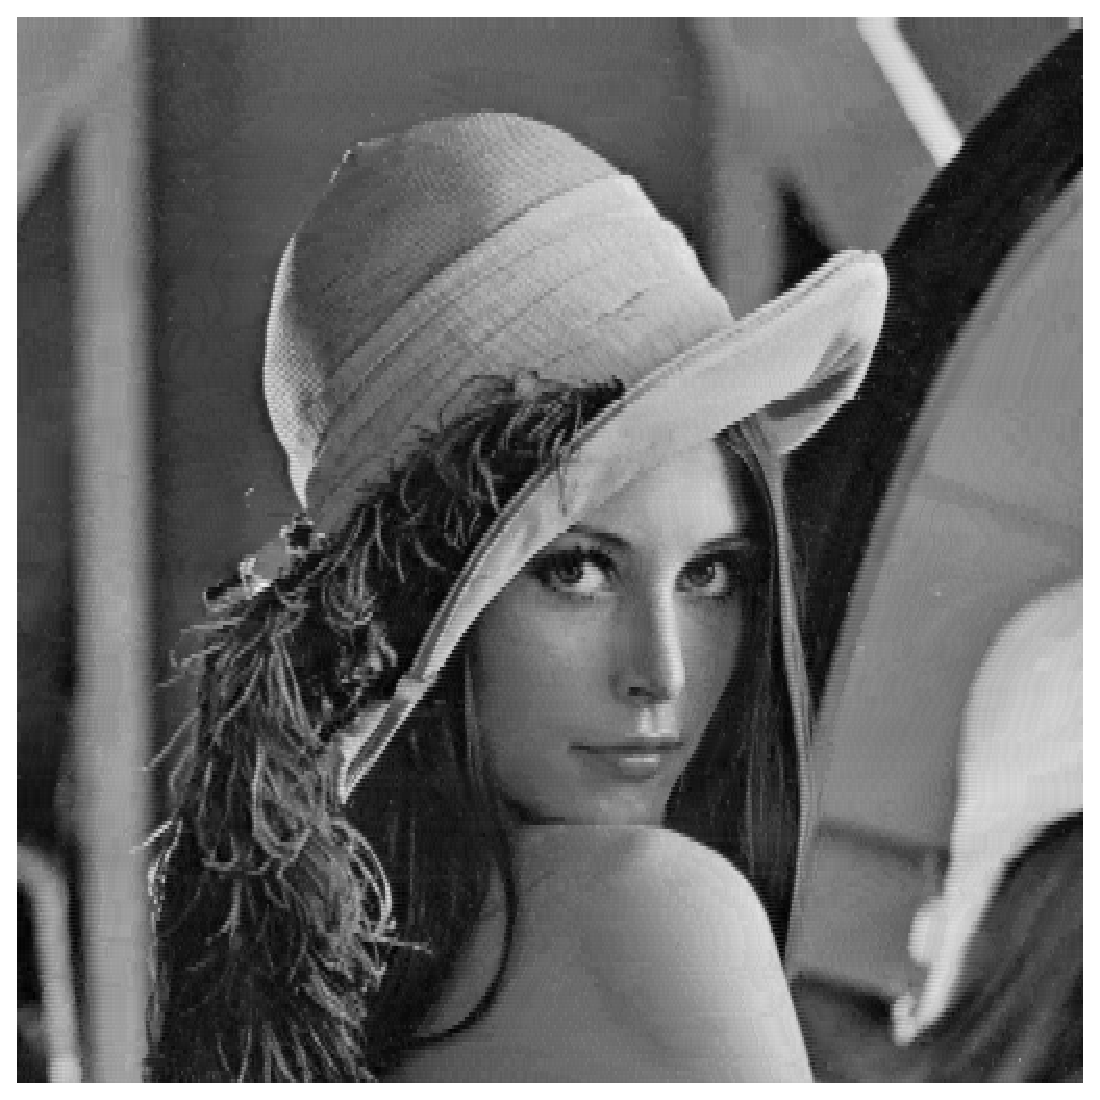
\psfig{file=lena_2b2.ps,width=2in}
    \psfig{file=lena_trans.ps,width=2in}
    }
  \centerline{(c)\hspace{2cm}(d)}
  \centerline{\Large Figure 1: Different flavors of PMIC on the ``Lena'' image}
  Comparisons of different flavors of PMIC on the ``Lena'' image:
(a) Classical PMIC (compression ratio equal to 4.3);
(b) JPEG (compression ratio equal to 7.9);
(c) PMIC with simple predictive coding (compression ratio equal to 7.9);
(d) PMIC with column compression (compression equal to 5.3).
\end{htmlonly}

As mentioned above, in this paper we investigate an impact of
prediction algorithms on PMIC. A simple prediction enhancement can
work as follows (prediction loop -- our main contribution of
this paper -- is described in depth in next sections):\\

{\bf Prediction}. A significant speed up in compression without major
deterioration in quality can be obtained by using prediction. It works as
follows: we compressed only every second row of an image, and when
decompressed we restore the missing row by using a prediction (cf.
\cite{rj}, and next sections).  For high quality image compression, one can
design a two-rounds approach where in the second round one sends the
missing rows.  Figure~\ref{comp_lena_flavors} shows two versions of the
compressed Lena picture: one with PMIC, and the other with PMIC and
predictive ``reduction/expansion''.\\

Finally, we also explore in this paper one more feature, namely:\\

{\bf Column compression}. PMIC is performed on rows. 
In order to have it performed on columns,
one simple way to proceed is to ``transpose'' the original image before
compression. Indeed, the rows of the compressed ``transposed''
image are the columns of the original one. This algorithm has been
performed on several different images, and this feature can sometimes
increase either the compression ratio or the quality level, as shown in
Figure~\ref{comp_lena_flavors}.\\

Let us discuss algorithmic challenges of PMIC. It boils down to
an efficient implementation of finding the longest prefix of length $L_n$
in yet uncompressed file. 
We present below one possible implementation (for others the
reader is refereed to \cite{ags}.
Let $x_1^n$ denote the database, $y_1^m=x_{n+1}^{n+m}$ denote the
yet uncompressed file.
As before, we write $d(x_i,y_j)$ for a distortion measure between two
symbols, where $d( \cdot , \cdot )$ is understood to incorporate
the max-difference criterion discussed earlier.\\

{\bf Algorithm} {\tt PREFIX}\\
{\bf Input:} $x_1^n$ and $y_1^m$\\
{\bf Output:} Largest integer $k$ such that, for some index $t$ ($1
\leq t \leq n-m$),
$d ( x_t^{t+k-1} , y_1^k ) \leq D$.  The algorithm outputs both $k$
and $t$.\\
{\bf Method:} We compute, for all $i,j$ $S_{ij}$ $=$ total distortion
measure between $x_i^{i+j-1}$ and $y_1^j$.\\

\begin{tabbing}
{\bf begin}\=  \\
         \> Initialize all $S_{ij} := 0$.\\
         \> {\bf for} \= $i=1$ {\bf to} $n-m$ {\bf do} \\
         \> \> {\bf for} \= $j=1$ {\bf to} $m$ {\bf do} \\
         \>  \>  \> Compute $S_{ij} := S_{i,j-1} + d(x_{i+j-1}, y_j)$\\
         \>  \> {\bf doend} \\
         \>  {\bf doend} \\
         \>  Let $k$ be the largest $j$ such that $S_{ij} \leq j D$,
         and let $t$ be the corresponding $i$\\
         \>  {\bf Output} $k$ and $t$\\
{\bf end}
\end{tabbing}

The above can easily be modified to incorporate the enhancements
discussed above (additive shift, etc.) and to use $O(1)$ variables
rather than the $S_{ij}$ array.\\

%In one of our implementation, 
%an image $N\times N$ is compressed in $O(N^2\log N)$ when the
%database string is of length $m=O(1)$.

In order to compress an $N\times N$ image we apply {\tt PREFIX} several
times to compress a row, which we call {\tt COMPRESS\_\,ROW} algorithm,
and this is further use to compress a whole image in either
{\tt COMPRESS\_\,LONG\_\,DATABASE} (where the database sequence is of
multiplicity of $N$, i.e., $f N$ where $f$ is a small integer)
or {\tt COMPRESS\_\,SHORT\_\,DATABASE} (where the database sequence is
of length $O(1)$ but located just above the ``point'' of compression). 
In the former case the algorithmic complexity of
compression is $O(N^4)$ while in the latter case it is $O(n^2\log N)$ which
is only $\log N$ away from the optimal complexity $O(N^2)$. 
In this paper we only use {\tt COMPRESS\_\,SHORT\_\,DATABASE} algorithm.

\section{Review of DPCM}

In the following, $x_{i,j} = \xm$ stands for the color value of the pixel
currently in position $(i,j) = m$ in the $N\times N$ pixels original
image, and $\xh_{i,j} = \xmh$ is the color value of the ``predicted''
(reconstructed) pixel of the reconstructed image. As seen in \cite{rj}
and accordingly to Fig.~\ref{pred_cfg}, the configuration of the 2-D
predictor is as following:

\begin{figure}[htbp]
  \centerline{
    \psfig{file=DPCM_predictor_config.epsi,width=4in,angle=-90}
    }
  \caption{DPCM predictor configuration.}
  \label{pred_cfg}
\end{figure}

\begin{equation}
  \xmh = 0.75A - 0.50B + 0.75C.
  \label{x_def}
\end{equation}

where $\xm = x_{i,j}$, $A = \xh_{i,j-1}$, $B = \xh_{i-1,j-1}$, and
$C = \xh_{i-1,j}$.\\

In the above, $e_m$ stands for the error value between the original and the
reconstructed pixels:

\begin{equation}
e_m = \xm - \xmh.
\end{equation}

Finally, $\ems$ is the quantized value of $e_m$, as described in
\cite{rj} from which Table~\ref{8_level_quantizer_t} is drawn.
Then:\\

{\bf Algorithm} {\tt PREDICTION}\\
{\bf Input:} $x_{i,j} = \xm$, $\xh_{i,j-1} = A$, $\xh_{i-1,j-1} = B$, and
$\xh_{i-1,j} = C$ (see Fig.~\ref{pred_cfg}).\\
{\bf Output:} $\ems$.\\
{\bf Method:} We compute a first $\xmh$, then $e_m$ and
$\ems$. Eventually, we update the value of $\xmh$.\\

\begin{tabbing}
{\bf begin}\=  \\
        \> Compute $\xmh$ accordingly to Eq.~\ref{x_def} \\
        \> Clip $\xmh$ to the range [0,255] \\
        \> Compute $e_m := x_m - \xmh$ \\
        \> Compute $\ems := Quantize (e_m)$ \\
        \> Upgrade $\xmh$ by computing $\xmh$ := $\xmh + \ems$ \\
        \> Clip $\xmh$ to the range [0,255] \\
{\bf end}
\end{tabbing}
\noindent

\begin{table}[htbp]
\centerline{
\begin{tabular}{|c|c|c|c|}      \hline
i & $(d_i,d_{i+1}) \rightarrow r_i$ & Probability & Huffman Code \\ \hline
0 & (-255,-16) $\rightarrow$ -20 & 0.025 & 111111 \\ \hline
1 & (-16,-8) $\rightarrow$ -11 & 0.047 & 11110 \\ \hline
2 & (-8,-4) $\rightarrow$ -6 & 0.145 & 110 \\ \hline
3 & (-4,0) $\rightarrow$ -2 & 0.278 & 00 \\ \hline
4 & (0,4) $\rightarrow$ 2 & 0.283 & 10 \\ \hline
5 & (4,8) $\rightarrow$ 6 & 0.151 & 01 \\ \hline
6 & (8,16) $\rightarrow$ 11 & 0.049 & 1110 \\ \hline
7 & (16,255) $\rightarrow$ 20 & 0.022 & 111110 \\ \hline
\end{tabular}}
\caption{8-level Lloyd-Max quantizer for the ``Lena'' image.}
\label{8_level_quantizer_t}
\end{table}

In fact, we add an offset of 128 to $\ems$, making all of the error
values positive (for an 8-bit original) so that they can be printed on
a output device. The error image for a perfectly reconstructed image
is thus uniform gray field with a code value of 128.

\begin{figure}[htbp]
  \psfig{file=DPCM_block_diagram.epsi,width=5in,angle=-90}
  \caption{DPCM block diagram.}
  \label{DPCM_block_diagram}
\end{figure}

The DPCM algorithm is summarized in Figure~\ref{DPCM_block_diagram}. We
observe that it applies to every pixel of the image. That leads to the
following algorithm:\\

{\bf Algorithm} {\tt PREDICTION\_LOOP}\\
{\bf Input:} $x_{i,j} = \xm$, for all $(0\leq i\leq N-1)$ and $(0\leq
j\leq N-1)$.\\
{\bf Output:} $\ems$, for all $(0\leq i\leq N-1)$ and $(0\leq
j\leq N-1)$.\\
{\bf Method:} We use {\tt PREDICTION} to compute $\ems$ for each
pixel.
\begin{tabbing}
{\bf begin}\=  \\
        \> Initialize $\xmh = \xm$ and $\ems = \xm$ for all $(0\leq i\leq N-1)$ and $j=0$.\\
        \> {\bf for} \= $j=1$ {\bf to} $N-1$ {\bf do} \\
        \> \> {\bf for} \= $i=0$ {\bf to} $N-1$ {\bf do} \\
        \>  \>  \> {\bf Call} {\tt PREDICTION} on $x_{i,j} = \xm$, $\xh_{i,j-1} = A$, $\xh_{i-1,j-1} = B$, and\\
        \> \> \> $\xh_{i-1,j} = C$ (see Fig.~\ref{pred_cfg}).\\
        \>  \> {\bf doend} \\
        \>  {\bf doend} \\
{\bf end}
\end{tabbing}

From Figure ~\ref{DPCM_block_diagram} one concludes that the prediction
(reconstructed pixel) $\xmh$ for the transmitter is exactly the same as the
one used by the receiver. They both need, and only need, the quantized
difference $\ems$. The transmitter puts this difference in a file, whereas
the receiver reads this difference from the file.\\

Finally, $\ems$, which is the quantized difference for each pixel, and the
whole picture (formed with these quantized differences) is compressed with
Huffman code.

\section{New Algorithm: PMIC with DPCM}


Like in Huffman compression (the compression part of DPCM), the PMIC
compression algorithm should be performed on the quantized differential
image. However, the algorithms seen above are well adapted to Huffman
coding, because they deal on a pixel-by-pixel basis. Unfortunately, the
PMIC algorithm, proceeds several pixels at a time (i.e., the longest prefix
found in the database). Besides, we do not know in advance what the length
of this prefix will be. But, there is a way around all of those problems.
In fact, if we consider the {\tt PREDICTION} algorithm to be performed, not
on a pixel basis, but on a cell (which is, in the case of DPCM, one single
pixel) basis, then this algorithm needs just a few adaptations in order to
be suited for PMIC: in this latter, the cell becomes naturally the longest
prefix found in the database.\\

These considerations lead to the algorithms given below, which should
replace the {\tt PREFIX} and {\tt COMPRESS\_ROW} algorithms 
for more detail) respectively:\\

{\bf Algorithm} {\tt DIFFERENTIAL\_PREFIX}\\
{\bf Input:} $\xh_1^n$, $ex_1^n$ (where $n=fN$), and $y_1^N$\\
{\bf Output:} Largest integer $k$ such that, for some index $t$ ($1
\leq t \leq n-N$), $d ( ex_t^{t+k-1} , ey_1^k ) \leq D$. The algorithm
outputs both $k$ and $t$, as well as $\yh_1^N$ and $ey_1^N$, both
returned by the call to the {\tt PREDICTION\_LOOP} algorithm.\\
{\bf Method:} We first use {\tt PREDICTION\_LOOP} to form a
differential row, then we compute, for all $i,j$, $S_{ij}$ $=$ total
distortion measure between $ex_i^{i+j-1}$ and $ey_1^j$.
\begin{tabbing}
{\bf begin}\=  \\
        \> {\bf Call} {\tt PREDICTION\_LOOP} on $x_1^N$\\
        \> Let $\yh_1^N$ and $ey_1^N$ be returned by this call to {\tt PREDICTION\_LOOP}.\\
        \> Initialize all $S_{ij} := 0$.\\
        \> {\bf for} \= $i=1$ {\bf to} $n-N$ {\bf do} \\
        \> \> {\bf for} \= $j=1$ {\bf to} $N$ {\bf do} \\
        \>  \>  \> Compute $S_{ij} := S_{i,j-1} + d(ex_{i+j-1}, ey_j)$\\
        \>  \> {\bf doend} \\
        \>  {\bf doend} \\
        \>  Let $k$ be the largest $j$ such that $S_{ij} \leq j D$, and let $t$ be the corresponding $i$\\
        \>  {\bf Output} $k$ and $t$\\
{\bf end}
\end{tabbing}

One should note that the {\tt PREDICTION\_LOOP} algorithm is here used
on generally more pixels than needed, since it is used on $N$ pixels,
and that the longest prefix will have a size $\leq N$.\\

{\bf Algorithm} {\tt COMPRESS\_DIFFERENTIAL\_ROW}\\
{\bf Input:} $\xh_1^n$, $ex_1^n$ (where $n=fN$), $y_1^N$.\\
{\bf Output:} A compressed version of $ey_1^N$, in the form of
$(pointer,length)$ pairs, and the new reconstructed portion,
$\yh_1^N$, of the database.\\
{\bf Method:} We use {\tt PREFIX} to ``peel off'' a prefix
of the row being compressed, and repeat on the remaining
portion of that row until we use it all up.
\begin{tabbing}
{\bf begin}\=  \\
        \> Initialize $i := 0$.\\
        \> {\bf Repeat} \= the following {\bf until} $i \geq N$ \\
        \> \> {\bf Call} {\tt PREFIX} on $\xh_1^n$, $ex_1^n$ and $y_{i+1}^N$ \\
        \> \> Let $k$ and $t$, $\yh_{i+1}^N$ and $ey_{i+1}^N$, be returned by this call to {\tt PREFIX} \\
        \> \> {\bf If} $k$ is small (say, $\leq 4$) \\
        \> \> {\bf then} $ey_{i+1}^{i+k}$ is stored explicitly,\\
        \> \> {\bf else} $ey_{i+1}^{i+k}$ is stored as a $(pointer,length)$ pair,\\
        \> \> Compute $\yh_{i+1}^{i+k} := \yh_{i+1}^{i+k} +
        ey_{i+1}^{i+k}$ (addition of vectors).\\
        \> \> Set $i := i+k$\\
{\bf end}
\end{tabbing}

We have used here the notation $ex$ and $ey$ for $x$ and $y$, as they
are understood in the {\tt COMPRESS\_ROW} algorithm of \cite{ags} and
discussed briefly above, except that what
is now compressed is the quantized differential image, whence the $e$
before $x$ and $y$. Therefore, $\xh_1^n$ represents the reconstructed
(``predicted'') database (and is, in fact, the image as it will be
again after decompression); $ex_1^n$ means the database of the
differential image (image actually being compressed); $y_1^N$ is the
currently processed row of the original image; $ey_1^N$ is the
``differential'' row currently being compressed, that is, the
differential pendant of $y_1^N$; and $\yh_1^N$ is the new portion of
the reconstructed (``predicted'') database. Thus, $\yh$ leads to
$\xh$, and $ey$ gives $ex$.

\begin{table}[htbp]
\caption{``Lena'' image compressed by JPEG (quality=57), PMIC with
constant $D$ (D = 155, DD = 20), PMIC with variable $D$
(D1 = 500, D2 = 55, DD = 22), and PMIC-PL (D1 = 600, D2 = 50, DD = 16).}

\begin{center}
\begin{tabular}{|l|c|c|c|c|} \hline
& JPEG & Const D & Var D & PMIC-PL\\ \hline
Compression ratio & 10.03 & 9.99 & 10.01 & 10.04\\ \hline
Bit rate (bits/pixel) & 0.8 & 0.8 & 0.8 & 0.8\\ \hline
RMSE (0-255) & 4.65 & 8.90 & 8.44 & 15.97\\ \hline
PSNR (dB) & 34.78 & 29.14 & 29.61 & 24.06\\ \hline
\end{tabular}
\end{center}
\end{table}

\begin{table}[htbp]
\caption{``Basselope'' image compressed by JPEG (quality=57), PMIC with
constant $D$ (D = 800, DD = 38), PMIC with variable $D$
(D1 = 800, D2 = 100, DD = 39), and PMIC-PL (D1 = 1000, D2 = 45, DD = 15).}

\begin{center}
\begin{tabular}{|l|c|c|c|c|} \hline
& JPEG & Const D & Var D & PMIC-PL\\ \hline
Compression ratio & 9.96 & 10.04 & 10.04 & 9.96\\ \hline
Bit rate (bits/pixel) & 0.8 & 0.8 & 0.8 & 0.8\\ \hline
RMSE (0-255) & 9.07 & 12.22 & 8.44 & 78.89\\ \hline
PSNR (dB) & 28.97 & 26.39 & 29.61 & 10.19\\ \hline
\end{tabular}
\end{center}
\end{table}

\begin{table}[htbp]
\caption{``Lena'' image compressed by JPEG (quality=21), PMIC with
constant $D$ (D = 400, DD = 38), PMIC with variable $D$ 
( D1 = 500, D2 = 55, DD = 22), and PMIC-PL (D1 = 600, D2 = 50, DD = 16).}
\med
\begin{center}
\begin{tabular}{|l|c|c|c|c|} \hline
& JPEG & Const D & Var D & PMIC-PL\\ \hline
Compression ratio & 10.03 & 10.00 & 9.95 & 10.02\\ \hline
Bit rate (bits/pixel) & 0.8 & 0.8 & 0.8 & 0.8\\ \hline
RMSE (0-255) & 7.96 & 13.92 & 12.87 & 20.41\\ \hline
PSNR (dB) & 30.11 & 25.26 & 25.94 & 21.94\\ \hline
\end{tabular}
\end{center}
\end{table}

Finally, we present some experimental results. We summarize them in Tables
2---4 where JPEG, PMIC with constant and variable $D$, and PMIC-PL (PMIC
with Prediction Loop) are compared for three images, namely: ``Lena''
image, ``Basselope'' image (a graphic image) and ``San Francisco'' image (a
photographic image).  We conclude that prediction, as discussed in Section
2, can lead to substantial speed up of compression time, butter compression
time without significant deterioration of image quality. More sophisticated
PMIC-PL cna lead to further improvements, as our preliminary results
suggest. However, results in Tables 2-4 are, in fact, worse than
expected. We believe they originate from the fact that we use variable-D
scheme which seems to be unsuited for the predictive loop (the derivative
is actually done on the original image, and not on the differential image,
as it should be). This might be an interesting point further research
(\ie, to implement a good derivative scheme on the differential image).
Then, we believe we can achieve much more substantial improvements. This
will be reported in our journal version of this paper.

\small

\begin{thebibliography}{99}

\footnotesize


\bibitem{habibi} 
A. Habibi, 
Comparison of $n$th-order DPCM encoder
with linear transformations and block quantization techniques, 
{\it IEEE Trans. Commun. Tech}., COM-19, 948-956 (1971).
\bibitem{ags}
M. Atallah, Y. Genin, and W. Szpankowski,
A Pattern Matching Approach to Image Compression,
{\it Proc. International Conference on Image Processing}, vol. II,  349-352,
Lausanne (1996); see also
Purdue University, CSD-TR-95-083 (1995).
\bibitem{berger}
T. Berger,
{\it Rate Distortion Theory: A Mathematical Basis for Data Compression},
Englewood Cliffs, NJ: Prentice-Hall, 1971.
\bibitem{cs}
C. Constantinescu and J. Storer,
Improved Techniques for Single-Pass Adaptive Vector
Quantization, {\it Proc. of the IEEE}, 82, 933-939 (1994).
\bibitem{cr}
M. Crochemore and W. Rytter,
{\it Text Algorithms}, Oxford University Press, New York  (1995).
\bibitem{fck}
W. Finamore, M. Carvalho, and J. Kieffer,
Lossy Compression with the Lempel-Ziv Algorithm,
{\it 11th Brasilian Telecommunication Conference}, 141-146 (1993).
\bibitem{jain}
A. K. Jain,
{\it Fundamentals of Digital Image Processing}, Prentice-Hall,
Englewood (1989)
\bibitem{lus1}
T. \L uczak and W. Szpankowski,
A Lossy Data Compression Based on String Matching: Preliminary
Analysis and Suboptimal Algorithms,
{\it Proc. Combinatorial Pattern Matching}, Asilomar,
LNCS 807, 102-112, Springer-Verla  (1994).
\bibitem{lus2}
T. \L uczak and W. Szpankowski,
A Suboptimal Lossy Data Compression Based in Approximate Pattern Matching,
{\it IEEE International Symposium on Information Theory}, Whistler, 1995;
also under revision in {\it IEEE Trans. Information Theory},
and Purdue University, CSD-TR-94-072 (1994).
\bibitem{nl} 
A. N. Netravali and J. O. Limb, 
Picture Coding~: A Review,
{\it Proc. IEEE}, 68, 366-406 (1980).
\bibitem{rj}
M. Rabbani and P. Jones,
{\it Digital Image Compression Techniques}, SPIE Optical Engineering Press,
Bellingham (1991).
\bibitem{sn} 
D. K. Sharma and A. N. Netravali, 
Design of Quantizers for DPCM Coding of Picture Signals, 
{\it Proc. IEEE Trans. Commun.}, COM-25, 1267-1274 (1978).
\bibitem{sg}
Y. Steinberg and M. Gutman,
An Algorithm for Source Coding Subject to a Fidelity Criterion,
Based on String Matching,
{\it IEEE Trans. Information Theory}, 39,  877-886 (1993).
\bibitem{spa2}
W. Szpankowski,
A Generalized Suffix Tree and Its (Un)Expected Asymptotic Behaviors,
{\it SIAM J. Computing}, 22, 1176-1198  (1993).
\bibitem{wz}
A. Wyner and J. Ziv,
Some Asymptotic Properties of the Entropy of a Stationary Ergodic Data Source
with Applications to Data Compression,
{\it IEEE Trans. Information Theory}, 35, 1250-1258  (1989).
\bibitem{yk}
E.H. Yang, and J. Kieffer,
On the Performance of Data Compression Algorithms Based upon String Matching,
preprint (1995).
\bibitem{zl1}
J. Ziv and A. Lempel,
A Universal Algorithm for Sequential Data Compression, {\it IEEE
Trans. Information Theory}, 23, 3, 337-343 (1977).
\bibitem{zl2}
J. Ziv and A. Lempel,
Compression of Individual Sequences via Variable-rate Coding,
{\it IEEE Trans. Information Theory}, 24, 530-536, 1978.


\end{thebibliography}

\end{document}

